% 2003 年辽宁卷第 17 题：正四棱柱立体几何图
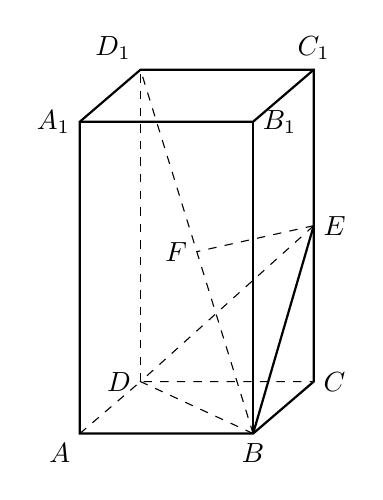
\begin{tikzpicture}[>=stealth,scale=1.1]
  % Coordinates
  \coordinate (A) at (0,0);
  \coordinate (B) at (2,0);
  \coordinate (C) at (2.7,0.6);
  \coordinate (D) at (0.7,0.6);

  \coordinate (A1) at (0,3.6);
  \coordinate (B1) at (2,3.6);
  \coordinate (C1) at (2.7,4.2);
  \coordinate (D1) at (0.7,4.2);

  \coordinate (E) at (2.7,2.4); % midpoint of CC1
  \coordinate (F) at (1.35,2.1); % midpoint of BD1

  % Solid edges
  \draw[thick] (A) -- (B) -- (C) -- (C1) -- (D1) -- (A1) -- cycle;
  \draw[thick] (A1) -- (B1) -- (C1);
  \draw[thick] (B) -- (B1);
  \draw[thick] (B) -- (E);

  % Dashed edges
  \draw[dashed] (A) -- (D) -- (C);
  \draw[dashed] (D) -- (D1);
  \draw[dashed] (B) -- (D1);
  \draw[dashed] (B) -- (D) -- (E);
  \draw[dashed] (E) -- (F);

  % Labels
  \node[below left] at (A) {$A$};
  \node[below] at (B) {$B$};
  \node[right] at (C) {$C$};
  \node[left] at (D) {$D$};
  \node[left] at (A1) {$A_1$};
  \node[right] at (B1) {$B_1$};
  \node[above] at (C1) {$C_1$};
  \node[above left] at (D1) {$D_1$};
  \node[right] at (E) {$E$};
  \node[left] at (F) {$F$};
\end{tikzpicture}
